% -----------------------------------------------------------------------------

\begin{frame}{Brain PCoA}
    \begin{columns}[c] % The "c" option specifies centered vertical alignment while the "t" option is used for top vertical alignment

        \column{.45\textwidth} % Left column and width
        \textbf{Details}
        \begin{itemize}
            \item PCA, Euclidean distance of brain regions, normalized by total brain size
            \item All kids with processed brain scans
            \item Top: colored by age, first 2 axes
            \item Bottom: PCA1 x Age, colored by cogscore
            
        \end{itemize}

        \column{.5\textwidth} % Right column and width
    
        \begin{figure}
        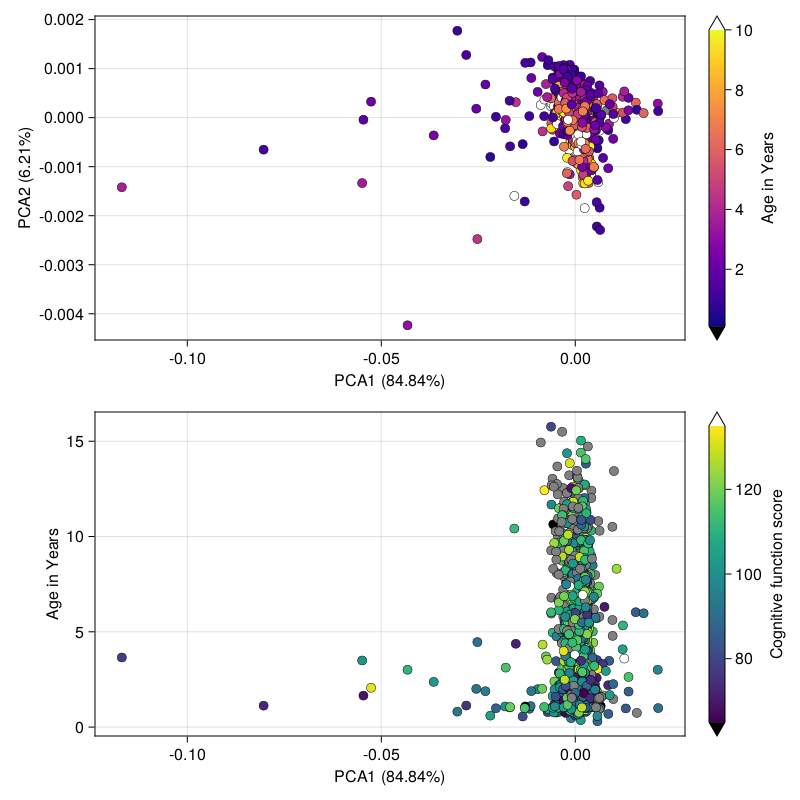
\includegraphics[width=1\linewidth]{../figures/brain_pcoa.png}
        \end{figure}

    \end{columns}
\end{frame}

% -----------------------------------------------------------------------------

\begin{frame}{Cognitive score summaries}
    \begin{columns}[c] % The "c" option specifies centered vertical alignment while the "t" option is used for top vertical alignment

        \column{.45\textwidth} % Left column and width
        
        \begin{figure}
            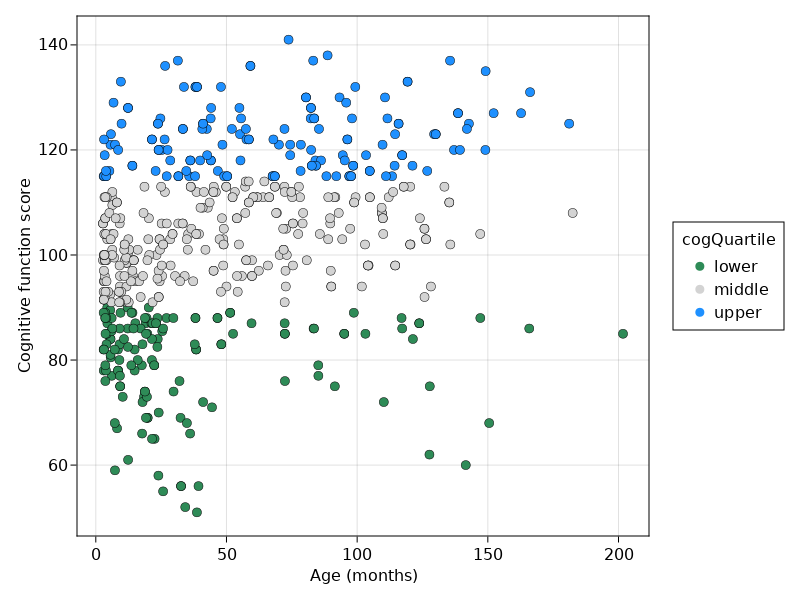
\includegraphics[width=1\linewidth]{../figures/cogScore_quartiles.png}
        \end{figure}

        \column{.5\textwidth} % Right column and width
    
        \begin{figure}
        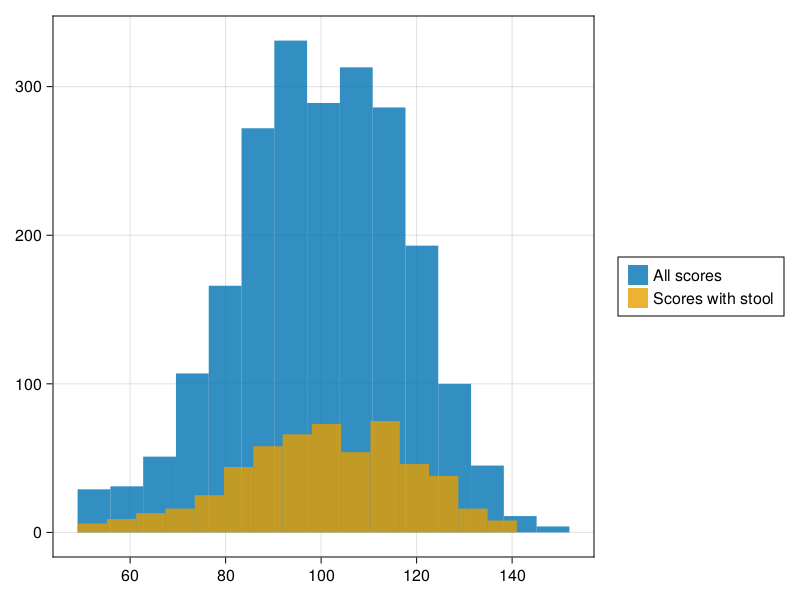
\includegraphics[width=1\linewidth]{../figures/cogscores_hist.pdf}
        \end{figure}

    \end{columns}

    \textbf{Details}
    \begin{itemize}
        \item Quartiles calculated based on all measurements
    \end{itemize}

\end{frame}

% -----------------------------------------------------------------------------
